% !TEX root = task-3-21-1.tex
% Editable task bank. Append new BankTask blocks at the end of the document.
\documentclass[12pt,a4paper]{article}
\usepackage{physics-textbook}
\usepackage{graphicx,needspace}
\usetikzlibrary{decorations.pathmorphing}
\newif\ifShowSolutions
\ifdefined\TutorEdition
  \ShowSolutionstrue
\else
  \ShowSolutionsfalse % Change to \ShowSolutionstrue to display solutions.
\fi
\newcounter{banktask}
\newsavebox{\BankTaskBox}
\newcommand{\BankTaskContent}[3]{%
  \noindent\textbf{\thebanktask.}\quad #2\par
  \ifShowSolutions
    \Needspace{50mm}% Keep the solution heading with its opening text or diagram.
    #3\par
    \ifdefined\TutorEdition
      \ifcsname TutorSource#1\endcsname
        \nopagebreak\smallskip{\small\csname TutorSource#1\endcsname\par}%
      \fi
    \fi
  \fi
}
\newcommand{\BankTask}[3]{%
  \refstepcounter{banktask}\par\medskip
  \sbox{\BankTaskBox}{\begin{minipage}{\linewidth}%
    \BankTaskContent{#1}{#2}{#3}\end{minipage}}%
  \ifdim\dimexpr\ht\BankTaskBox+\dp\BankTaskBox\relax>\dimexpr\textheight-20mm\relax
    \Needspace{35mm}\BankTaskContent{#1}{#2}{#3}%
  \else
    \Needspace{\dimexpr\ht\BankTaskBox+\dp\BankTaskBox\relax}%
    \noindent\usebox{\BankTaskBox}\par
  \fi
  \medskip
}
\begin{document}
\BookSubsection{3.21.1}{Колебательный контур}


% Source sdamgia-1608: https://phys-ege.sdamgia.ru/problem?id=1608
\BankTask{sdamgia-1608}{
В наборе радиодеталей для изготовления простого колебательного контура имеются две катушки с индуктивностями $L_1 = 1\,\text{мкГн}$ и $L_2=2\,\text{мкГн},$ а также два конденсатора, емкости которых $C_1= 30\,\text{пФ}$ и $C_2= 40\,\text{пФ}.$ С какой наибольшей собственной частотой $\nu$ можно составить колебательный контур из двух элементов этого набора? (Ответ выразите в мегагерцах и округлите до целого числа.)
}{
\smallskip\noindent\textbf{Решение}\par
Частота собственных колебаний контура связана с емкостью конденсатора и индуктивностью катушки соотношением $\nu = \frac{1}{2 \pi \sqrt{LC}} .$ Таким образом, частота $\nu$ максимальна, когда LC минимально. Следовательно, необходимо выбрать $L_1$ и $C_1,$ при этом собственная частота контура составит:

\[\nu = \frac{1}{2 \cdot 3{,}14 \cdot \sqrt{1\cdot 10^{-6}\cdot 30\cdot 10^{-12}}} \approx29 \cdot 10 ^{6} \,\text{Гц}=29\,\text{МГц}.\]

Ответ: $29$.
}

% Source sdamgia-1626: https://phys-ege.sdamgia.ru/problem?id=1626
\BankTask{sdamgia-1626}{
Дан колебательный контур из конденсатора электроемкостью $50$ мкФ и катушки индуктивностью $2$ Гн. Какова циклическая частота свободных электромагнитных колебаний? (Ответ дать в $\frac{\,\text{рад}}{\,\text{с}}$ .)
}{
\smallskip\noindent\textbf{Решение}\par
Циклическая частота свободных электромагнитных колебаний в колебательном контуре связана с электроемкостью конденсатора и индуктивностью катушки соотношением: 

\[\omega = \frac{1}{\sqrt{LC}} = \frac{1}{\sqrt{2 \cdot 50 \cdot 10 ^{ - 6} }} =100 \frac{\,\text{рад}}{\,\text{с}} .\]

Ответ: $100$.
}

% Source sdamgia-3341: https://phys-ege.sdamgia.ru/problem?id=3341
\BankTask{sdamgia-3341}{
Колебательный контур состоит из катушки индуктивности и конденсатора. В нем наблюдаются гармонические электромагнитные колебания с периодом Т  =  $5\,\text{мс}$. В начальный момент времени заряд конденсатора максимален и равен $4 \cdot 10 ^{ - 6 } \,\text{Кл}.$ Каков будет заряд конденсатора через t  =  $2{,}5\,\text{мс}$? (Ответ дать в мкКл.)
}{
\smallskip\noindent\textbf{Решение}\par
Поскольку период колебаний равен $5\,\text{мс}$, через $2{,}5\,\text{мс}$ пройдет полпериода, а значит, конденсатор уже успеет разрядиться (за первую четверть периода) и перезарядиться в другом направлении (за вторую четверть). Следовательно, заряд конденсатора будет равен $4 \cdot 10 ^{ - 6 } \,\text{Кл}$ (но знаки зарядов пластин поменяются).

Ответ: $4$.
}

% Source sdamgia-11272: https://phys-ege.sdamgia.ru/problem?id=11272
\BankTask{sdamgia-11272}{
Колебательный контур состоит из катушки индуктивности и батареи конденсаторов. В состав батареи входят четыре одинаковых конденсатора, соединенных параллельно. Круговая частота \ensuremath{\omega} свободных электромагнитных колебаний, которые могут происходить в этом контуре, равна $2500\,\text{с}^{-1}$. По разным причинам три конденсатора из четырех вышли из строя. На сколько изменилась круговая частота свободных электромагнитных колебаний в контуре?
}{
\smallskip\noindent\textbf{Решение}\par
Общая емкость конденсаторов при параллельном соединении равна сумме емкостей всех соединенных конденсаторов. Таким образом, после выхода из строя трех конденсаторов электроемкость батареи конденсаторов уменьшится в $4$ раза.
Круговая частота колебательного контура рассчитывается по формуле: 

\[\omega= \frac{1}{\sqrt{LC}} ,\]

При уменьшении электроемкости в $4$ раза круговая частота колебательного контура увеличится в $2$ раза и станет равной $5000\,\text{с}^{-1}$. Таким образом, изменение составит $2500\,\text{с}^{-1}$.

Ответ: $2500$.
}

% Source sdamgia-24104: https://phys-ege.sdamgia.ru/problem?id=24104
\BankTask{sdamgia-24104}{
В идеальном колебательном контуре заряд q конденсатора емкостью $25$ пФ изменяется с течением времени t по закону $q=10 ^{ - 5 } \cos ( 10 ^{6} \cdot t )$ (в этой формуле все величины заданы в СИ). Какую максимальную энергию запасает катушка контура в процессе таких колебаний?
}{
\smallskip\noindent\textbf{Решение}\par
Из закона изменения заряда на конденсаторе следует, что максимальная энергия катушки с током равна максимальной энергии заряженного конденсатора. Из уравнения находим q$_{max}$  =  $10^{-5}$ Кл. Максимальная энергия конденсатора равна: 

\[W= \frac{q_{\max} ^2}{2C} = \frac{10 ^{ - 10 }}{2 \cdot 25 \cdot 10 ^{ - 12 }} =2\,\text{Дж}.\]

Ответ: $2$.
}

% Source sdamgia-32070: https://phys-ege.sdamgia.ru/problem?id=32070
\BankTask{sdamgia-32070}{
Заряд q на одной из пластин конденсатора, включенного в идеальный колебательный контур, меняется с течением времени t по закону $q = 2 \cdot 10 ^{ - 9 } \sin ( 5 \cdot 10 ^{6} t ) ,$ где все величины выражены в единицах СИ. Чему равна максимальная сила тока в контуре? Ответ запишите в амперах.
}{
\smallskip\noindent\textbf{Решение}\par
Из уравнения колебаний заряда $q ( t ) =q_{\max} \sin ( \omega t )$ находим, что максимальное значение заряда равно $q_{\max}=2 \cdot 10 ^{ - 9 } \,\text{Кл},$ а циклическая частота $\omega=5 \cdot 10 ^{6} \,\text{рад/с}.$
Сила тока меняется по закону $i=q'_t=q_{\max}\omega \cos ( \omega t ) =I_{\max} \cos ( \omega t ) .$ Следовательно, максимальное значение силы тока:

\[I_{\max}=q_{\max}\omega=2 \cdot 10 ^{ - 9 } \cdot 5 \cdot 10 ^{6} =0{,}01\,\text{А}.\]

Ответ: $0{,}01$.
}

% Source sdamgia-32590: https://phys-ege.sdamgia.ru/problem?id=32590
\BankTask{sdamgia-32590}{
Период свободных колебаний тока в идеальном колебательном контуре равен $5\,\text{мкс}$. В некоторый момент времени энергия магнитного поля в катушке достигает минимума. Через какое минимальное время после этого достигнет минимума энергия электрического поля в конденсаторе? Ответ запишите в микросекундах.
}{
\smallskip\noindent\textbf{Решение}\par
Энергия магнитного поля катушки с током будет иметь минимальное значение, когда энергия электрического поля конденсатора максимальна. Энергия в конденсаторе примет минимальное значение через четверть периода, то есть через промежуток времени:

\[t= \frac{T}{4} = \frac{5}{4} =1{,}25\,\text{мкс}.\]

Ответ: $1{,}25$.
}

% Source sdamgia-16873: https://phys-ege.sdamgia.ru/problem?id=16873
\BankTask{sdamgia-16873}{
\begin{center}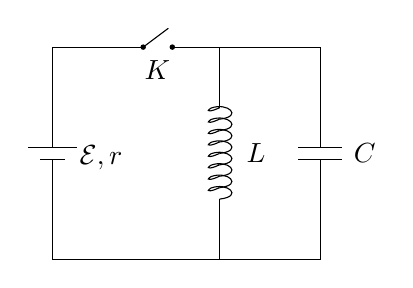
\begin{tikzpicture}[>=stealth]

\draw (0,0)--(3.4,0)--(3.4,1.27) (3.4,1.43)--(3.4,2.7)--(1.52,2.7) (1.15,2.7)--(0,2.7)--(0,1.43) (0,1.27)--(0,0)
(-.31,1.43)--(.31,1.43) (-.16,1.27)--(.16,1.27) (3.12,1.27)--(3.68,1.27) (3.12,1.43)--(3.68,1.43);
\draw(1.15,2.7)--(1.47,2.94);\fill (1.15,2.7)circle(.035) (1.52,2.7)circle(.035);
\node[below]at(1.33,2.65){$K$};\node[right]at(.22,1.30){$\mathcal E,r$};\node[right]at(3.7,1.35){$C$};
\draw (2.12,0)--(2.12,.77) (2.12,1.93)--(2.12,2.7);
\foreach \y in {.77,.915,1.06,1.205,1.35,1.495,1.64,1.785}{
 \begin{scope}[shift={(2.12,\y)}]\draw(0,0)..controls(.31,.035)and(.10,.22)..(-.11,.14)..controls(-.2,.08)and(-.08,.105)..(0,.145);\end{scope}}
\node[right]at(2.34,1.35){$L$};
\end{tikzpicture}\end{center}
В электрической цепи, показанной на рисунке, ключ К длительное время замкнут, $\mathcal E = 3\,\text{В},$ r = $2\,\text{Ом}$, L = $1$ мГн, С = $50$ мкФ. В момент t = $0$ ключ К размыкают. Каково напряжение U на конденсаторе в момент, когда в ходе возникших в контуре электромагнитных колебаний сила тока в контуре I = $1\,\text{А}$? Сопротивлением проводов и активным сопротивлением катушки индуктивности пренебречь.
}{
\smallskip\noindent\textbf{Решение}\par
Пока ключ замкнут через катушку течет постоянный ток $I_0,$ определяемый сопротивлением источника: $I_0 = \frac{\mathcal E}{r} .$ Поскольку активное сопротивление катушки, по условию, равно нулю, на катушке не падает напряжение, а значит, нулевое напряжение приложено к конденсатору. Таким образом, до размыкания ключа конденсатор разряжен. Начальная энергия электромагнитного поля в катушке $\frac{LI_0 ^2}{2} .$
После размыкания ключа начинаются электромагнитные колебания, и вся энергия, запасенная в катушке, будет перетекать из катушки в конденсатор и обратно. Энергия конденсатора равна $\frac{CU ^2}{2} .$ Через некоторое время энергия катушки уменьшится, а энергия конденсатора увеличится, причем сумма этих энергий будет равна начальной энергии катушки:

\[\frac{LI_0 ^2}{2} = \frac{LI ^2}{2} + \frac{CU ^2}{2} .\]

Откуда:

\[U = \sqrt{\frac{L ( I_0 ^2 - I ^2 )}{C}} = \sqrt{\frac{10^{-3} \,\text{Гн} \cdot \bigl( ( \frac{3\,\text{В}}{2\,\text{Ом}} ) ^2 - ( 1\,\text{А} ) ^2 \bigr)}{50 \cdot 10 ^{ - 6 } \,\text{Ф}}} = 5\,\text{В}.\]

Ответ: $5\,\text{В}$.
}

% Source sdamgia-32270: https://phys-ege.sdamgia.ru/problem?id=32270
\BankTask{sdamgia-32270}{
В колебательном контуре, активное сопротивление которого равно нулю, происходят свободные электромагнитные колебания с периодом T  =  $50{,}24\,\text{мкс}$ и максимальным напряжением на конденсаторе $U_{max}$. Зависимость энергии электрического поля конденсатора от разности потенциалов между его обкладками в пределах от $0$ до $U_{max}$ приведена на графике. Определите максимальное значение силы тока в контуре.

\begin{center}\begin{tikzpicture}[>=stealth,line width=.65pt]\draw[step=.4,gray!50] (0,0)grid(4,4);\draw[->](0,0)--(5.15,0)node[below]{$U$, В};\draw[->](0,0)--(0,4.65)node[left]{$E_{\text{эл}}$, мДж};\node[below left]at(0,0){$0$};\node[left]at(0,2){$0{,}5$};\node[left]at(0,4){$1{,}0$};\node[below]at(2,0){$100$};\node[below]at(4,0){$200$};\draw[orange!80!black,domain=0:4,samples=55]plot(\x,{.2*\x*\x});\fill[orange!80!black](4,3.2)circle(.045);\end{tikzpicture}\end{center}
}{
\smallskip\noindent\textbf{Решение}\par
$1$.  По закону сохранения энергии при отсутствии активного сопротивления в колебательном контуре максимальная энергия заряженного конденсатора равна максимальной энергии магнитного поля катушки с током $W_p=W_{\,\text{м}}.$
При этом максимальная энергия катушки с током равна $W_{\,\text{м}}= \frac{LI ^2 _{\max}}{2} .$
$2$.  В условии задачи известен период колебаний. Период колебаний в колебательном контуре $T=2 \pi \sqrt{LC} .$
$3$.  Максимальная энергия заряженного конденсатора равна $W_{\,\text{р}}= \frac{CU_{\max} ^2}{2} .$
Тогда выражаем:

$C= \frac{2W_{\,\text{р}}}{U_{\max} ^2} ;$
$L= \frac{T ^2}{4 \pi ^2 C} ;$
$I_{\max}= \sqrt{\frac{2W_{\,\text{м}}}{L}} = \frac{4 \pi W_p}{TU_{\max}} .$

Из графика находим, что максимальное значение энергии электрического поля конденсатора $W_p=0{,}8 \cdot 10 ^{ - 3 } \,\text{Дж},$ максимальное напряжение на обкладках конденсатора $U_{\max}=200\,\text{В}.$ При подстановке значений в формулу получаем:

\[I_{\max}= \frac{4 \cdot 3{,}14 \cdot 0{,}8 \cdot 10 ^{ - 3 }}{50{,}24 \cdot 10 ^{ - 6 } \cdot 200} =1\,\text{А}.\]

Ответ: $1\,\text{А}$.
}

% Source sdamgia-4508: https://phys-ege.sdamgia.ru/problem?id=4508
\BankTask{sdamgia-4508}{
К колебательному контуру подсоединили источник тока, на клеммах которого напряжение гармонически меняется с частотой $\nu.$ Электроемкость С конденсатора колебательного контура можно плавно менять от минимального значения $C_{\min}$ до максимального $C_{\max},$ а индуктивность его катушки постоянна. Ученик постепенно увеличивал емкость конденсатора от минимального значения до максимального и обнаружил, что амплитуда силы тока в контуре все время возрастала. Опираясь на свои знания по электродинамике, объясните наблюдения ученика.
}{
\smallskip\noindent\textbf{Решение}\par
В колебательном контуре источником тока возбуждаются вынужденные колебания. Частота этих колебаний равна частоте источника $\nu.$ Амплитуда же зависит от соотношения между внешней частотой и частотой собственных электромагнитных колебаний $\nu_0 = \frac{1}{2 \pi \sqrt{LC}} .$ По мере увеличения емкости конденсатора уменьшается частота собственных колебаний в колебательном контуре. Амплитуда колебаний достигает максимума при резонансе, когда $\nu=\nu_0.$ После этого амплитуда начинает убывать. В данном случае, ученик меняет не внешнюю частоту, а частоту собственных электромагнитных колебаний. При плавном увеличении емкости контура от минимального значения $C_{\min}$ до максимального $C_{\max},$ частота уменьшается от $\nu_0,\max = \frac{1}{2 \pi \sqrt{LC_{\min}}}$ до $\nu_0,\min = \frac{1}{2 \pi \sqrt{LC_{\max}}} .$ Из того факта, что амплитуда все время увеличивалась, можем сделать вывод, что частота $\nu_0$ все время приближалась к частоте источника тока, при этом $\nu < \nu_0,\min.$
}


% Source 70B4D7: https://ege.fipi.ru/bank/questions.php?search=1&proj=BA1F39653304A5B041B656915DC36B38&qid=70B4D7
\BankTask{70B4D7}{
Ученику необходимо обнаружить зависимость периода свободных электромагнитных колебаний в колебательном контуре от индуктивности катушки. Какие два колебательных контура он должен выбрать для проведения такого опыта?

\begin{center}
\begin{tikzpicture}[book diagram, x=1cm, y=1cm]
\foreach \x/\n/\ind/\cap in {0/1/{2L}/{C},3/2/{L}/{C},6/3/{L}/{2C},9/4/{2L}/{3C},12/5/{\dfrac{L}{2}}/{\dfrac{C}{2}}} {
\begin{scope}[shift={(\x,0)}]
\node at (0.5,-0.45) {\n)};
\draw (0,0.28)--(0,0)--(1,0)--(1,0.66);
\draw (0,1.09)--(0,1.4)--(1,1.4)--(1,0.82);
\draw plot[domain=0:1800,samples=241,variable=\t] ({0.10*sin(\t)},{0.235+0.81*\t/1800+0.045*cos(\t)});
\draw (0.74,0.66)--(1.26,0.66);
\draw (0.74,0.82)--(1.26,0.82);
\node[anchor=east] at (-0.15,0.7) {$\ind$};
\node[anchor=west] at (1.3,0.74) {$\cap$};
\end{scope}
}
\end{tikzpicture}
\end{center}
}{
\smallskip\noindent\textbf{Решение от GPT}\par
По формуле Томсона $T=2\pi\sqrt{LC}$, поэтому для исследования зависимости периода от индуктивности необходимо изменять $L$ при постоянной ёмкости. В контурах 1 и 2 ёмкость одинакова и равна $C$, а индуктивности равны $2L$ и $L$; следовательно, $T_1/T_2=\sqrt{2}$. В контурах 3, 4 и 5 ёмкости равны соответственно $2C$, $3C$ и $C/2$, поэтому они не образуют подходящей пары с одинаковой ёмкостью. Ответ: 12.
}

\end{document}
